\chapter{Task2}
\section{a)}
If we chose the machine $M$ as follows: $$M = (q_0, \emptyset, \delta, q_0, {q_0})$$
Then it can be proved that the only language accepted by a machine which has only the start state is the empty string $\epsilon$. 
So the second machine would have as complement language $$\Sigma^* \backslash \epsilon \rightarrow \epsilon \backslash \epsilon = \emptyset$$ remembering that $\emptyset^* = \epsilon$.\\
 So this would mean that the machine $M'$ would be something similar to this. 
\begin{center}
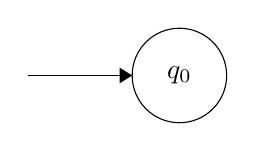
\begin{tikzpicture}[scale=0.2]
\tikzstyle{every node}+=[inner sep=0pt]
\draw [black] (25.5,-26.5) circle (3);
\draw (25.5,-26.5) node {$q_0$};
\draw [black] (15.9,-26.5) -- (22.5,-26.5);
\fill [black] (22.5,-26.5) -- (21.7,-26) -- (21.7,-27);
\end{tikzpicture}
\end{center}
Thus meaning that no language could be accepted by this machine. Since also $M'$ has like acceptance state $Q \backslash F \rightarrow q_0 \backslash q_0 \rightarrow \emptyset$. 
\section{b)}
\newpage
\section{c)}
	\begin{figure}[hbt]
	\label{L1}
  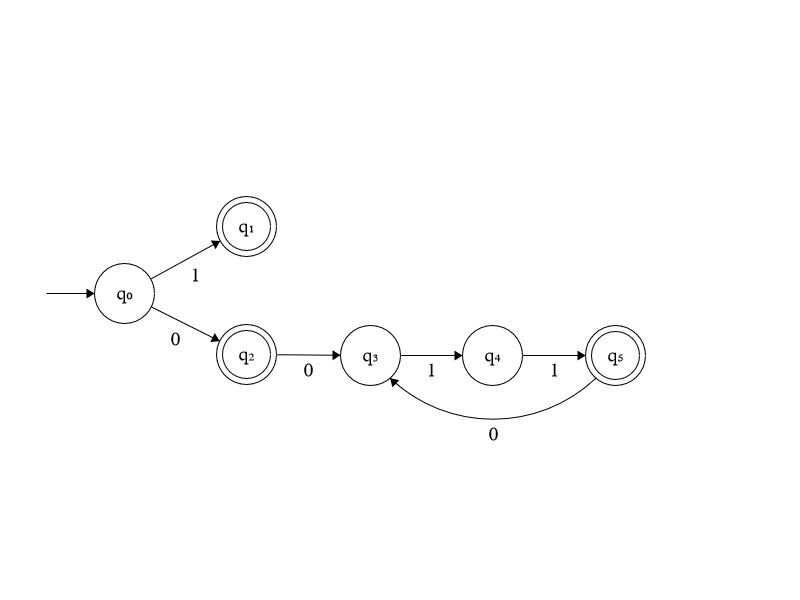
\includegraphics[width=\textwidth]{Immagini/l1.jpeg}
  \caption{L1}
\end{figure}



\begin{figure}[hbt]
	\label{L2}
  %\includegraphics[width=\textwidth]{Immagini/l2.jpeg}
  \caption{L2}
\end{figure}

